\documentclass[12pt,a4paper]{article}
\usepackage{geometry} % Adjust page margins
\geometry{margin=1in}
\usepackage{graphicx} % For including images
\usepackage{amsmath, amssymb} % For mathematical equations
\usepackage{hyperref} % For hyperlinks
\usepackage{booktabs} % For tables
\usepackage{caption} % For better captions
\usepackage{subcaption} % For subfigures
\usepackage{enumitem} % For custom lists
\usepackage{fancyhdr} % For header and footer
\usepackage{titlesec} % For section formatting
\usepackage{tocbibind} % To include TOC in the PDF

% Formatting headers and footers
\pagestyle{fancy}
\fancyhead[L]{Market Pulse: Stock Trend Prediction}
\fancyhead[R]{WIDS 4-Week Project}
\fancyfoot[C]{\thepage}

% Title Formatting
\title{\textbf{Market Pulse: Stock Trend Prediction Using Multivariate LSTM and Sentiment Analysis}}
\author{Rishith Gupta(23B1234) \\ WIDS 4-Week Project}
\date{\today}

\begin{document}

\maketitle
\newpage

% Table of Contents
\tableofcontents
\newpage

% Introduction
\section{Introduction}
Stock market prediction has been a long-standing challenge in financial markets, requiring the use of advanced techniques to understand trends and forecast future movements. Traditional statistical methods have given way to machine learning models, which leverage large datasets to extract meaningful patterns. Among these, deep learning models like Long Short-Term Memory (LSTM) networks have shown significant promise due to their ability to capture temporal dependencies in sequential data.

Moreover, financial markets are influenced not only by numerical indicators but also by public sentiment. News articles, social media discussions, and analyst opinions can heavily sway stock prices. Sentiment analysis, a Natural Language Processing (NLP) technique, helps quantify market sentiment and integrate it with stock price predictions. By combining multivariate LSTM models with sentiment analysis, we aim to improve the predictive accuracy of stock trends, providing valuable insights to investors and traders.

This project explores how multivariate LSTM models, enhanced with sentiment analysis, can predict stock market trends more effectively. The following sections will outline the theoretical background, methodology, implementation, and results of this approach.

\section{Week 0 : Introduction to time series and Python}
The project kicked off with learning Python, the language we would use to implement our final model. Alongside this, an introduction to time series analysis was essential to grasp the fundamentals of stock price prediction.

The assignment for this week focused on identifying trends and patterns in stock price and trading volume. This required exploring the yfinance library, which connects to Yahoo Finance and provides essential stock market data, including opening and closing prices, volume, adjusted closing prices, and daily highs and lows. For my analysis, I chose NASDAQ and examined five years of historical data.

Before diving into analysis, the data needed preprocessing to ensure the correct format, type, and structure. This involved handling missing values, verifying data types, and computing basic statistics. I then created various visualizations, including trading volume and closing price trends over time, and compared them with the 30-day moving average. This exploratory data analysis (EDA) helped uncover key patterns and insights.

Over the past five years, the closing prices have shown a steady upward trend, climbing from 6000 to 16,000. While the overall trajectory is positive, short-lived price spikes often lead to brief corrections before the stock resumes its upward movement. The presence of minor fluctuations, or "noise," can be smoothed out using rolling averages to reveal broader market patterns. Interestingly, no clear seasonal trends were observed in the data.

Trading volume initially remained stable but saw a sharp rise in the last two years, maintaining a higher average level. This surge in activity coincided with a significant price increase, suggesting a potential relationship between trading volume and market movements. Compared to stock prices, volume data appeared noisier, making it more challenging to interpret without applying smoothing techniques.

\begin{figure}[!h]
    \centering
    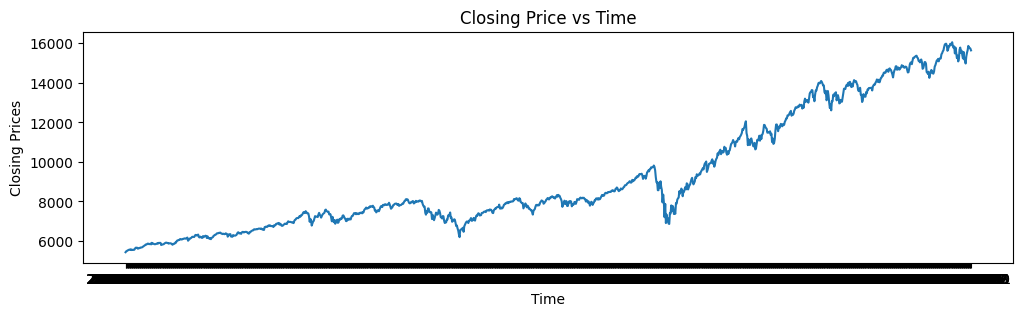
\includegraphics[width=0.8\textwidth]{Week0_closing_price.png} % Adjust width as needed
    \caption{Closing price vs time}
    \label{fig1}
\end{figure}

\begin{figure}[!h]
    \centering
    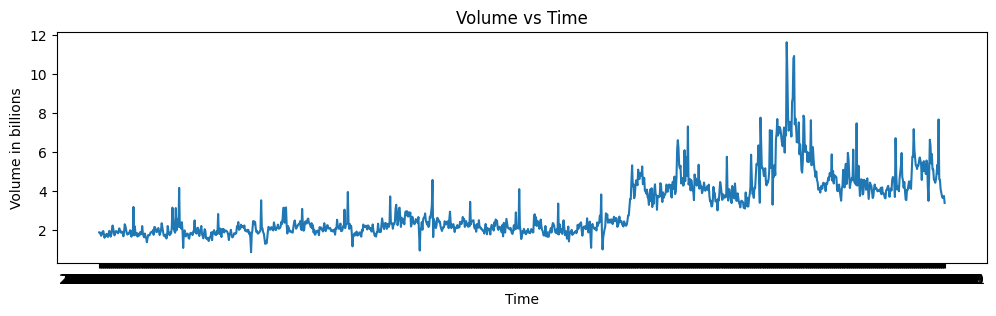
\includegraphics[width=0.8\textwidth]{Week0_volume.png} % Adjust width as needed
    \caption{Volume vs time}
    \label{fig2}
\end{figure}

\begin{figure}[!h]
    \centering
    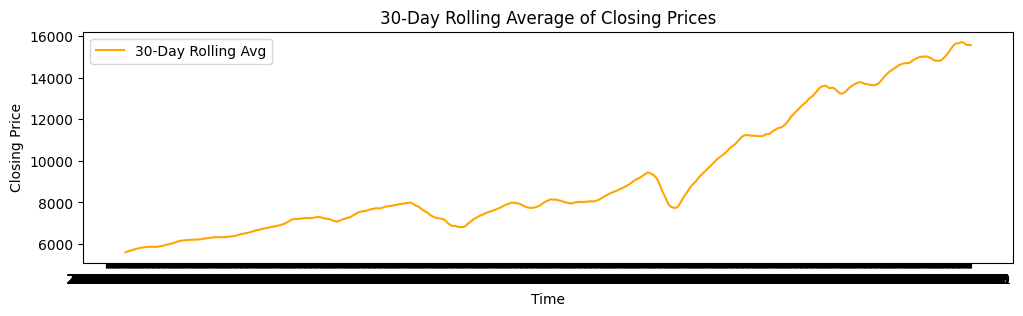
\includegraphics[width=0.8\textwidth]{Week0_30Rolling_average.png} % Adjust width as needed
    \caption{30 day rolling average of price vs time}
    \label{fig3}
\end{figure}

\section{Week 1 : Sentiment Analysis on text data}
This week focused on preparing stock data, extracting features, and understanding the role of sentiment analysis in financial forecasting. This required learning the basics of Natural Language Processing (NLP) and using TextBlob, a popular library for sentiment analysis.

TextBlob is a powerful yet easy-to-use NLP library built on top of NLTK and Pattern. It simplifies various text-processing tasks, making it widely used in sentiment analysis, text classification, and language translation. Key features include tokenization, noun phrase extraction, part-of-speech tagging, word inflection, and lemmatization. These functions help break down text into structured components, making analysis more effective.

One of the most valuable features of TextBlob is sentiment analysis, which quantifies the sentiment expressed in text. It provides two key metrics: polarity, which ranges from -1 (negative) to 1 (positive), and subjectivity, which indicates whether a statement is more factual or opinion-based. This makes it a useful tool for financial analysis, where market sentiment derived from news and social media can influence stock trends.

Additionally, TextBlob offers built-in spelling correction, making it useful for processing noisy datasets like social media posts. It also supports language detection and translation, allowing seamless text conversion across multiple languages. Another key functionality is text classification using a Naive Bayes classifier, which helps categorize text into predefined labels, such as positive or negative sentiment. The library also supports word frequency analysis and n-gram extraction, making it a versatile tool for NLP-based financial modeling.

This week’s assignment involved cleaning the IMDb dataset of top Netflix movies and TV shows in preparation for sentiment analysis. The preprocessing steps included removing rows with missing values and special characters. Since the dataset was already well-structured, minimal additional cleaning was required.

For sentiment analysis, the text data underwent further transformation, including removing stopwords, punctuation, escape sequences, special characters, HTML tags, URLs, and numbers. After preprocessing, lemmatization was applied, followed by sentiment analysis. The output consisted of two key values: polarity, which indicates whether the sentiment is positive or negative, and subjectivity, which measures how opinion-based the text is. These steps laid the foundation for integrating sentiment analysis into stock market forecasting.

\begin{figure}[!h]
    \centering
    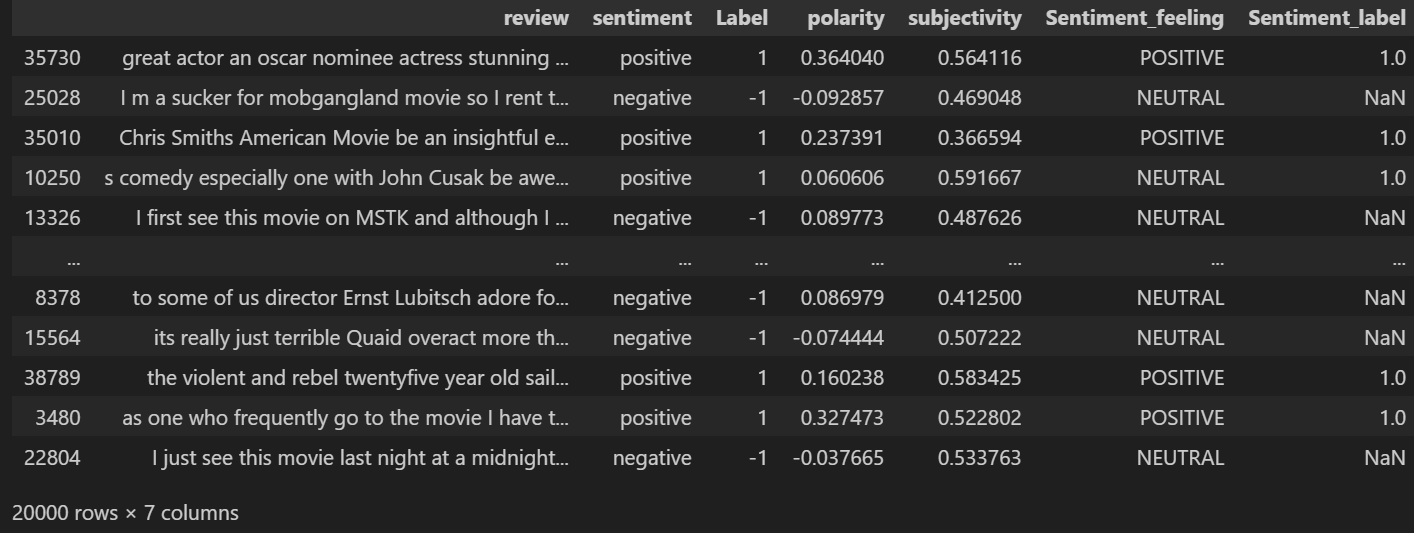
\includegraphics[width=0.8\textwidth]{Week1_Sentiment_results.png} % Adjust width as needed
    \caption{sentiment Analysis results}
    \label{fig4}
\end{figure}

\section{Week 2: Reinforcement Learning}
This week provided an introduction to the mathematical foundations of Reinforcement Learning. While this served as a stepping stone, the main focus was on ARIMA (Autoregressive Integrated Moving Average)—a widely used time series forecasting method for predicting future trends.

The first task was to implement a grid search to identify the optimal (p, d, q) parameters for ARIMA by comparing their Akaike Information Criterion (AIC) values. Once the best configuration was found, I proceeded to train the model on Microsoft's stock data, sourced from yfinance. Using a two-year training period, I forecasted the closing prices for the next 30 days.

To evaluate performance, I calculated Mean Absolute Error (MAE), Mean Squared Error (MSE), and Root Mean Squared Error (RMSE) for the forecasted period. The results were underwhelming, indicating that the model struggled to capture underlying patterns in the data. However, this experiment provided valuable insights and marked another step forward toward the final project.

\begin{figure}[!h]
    \centering
    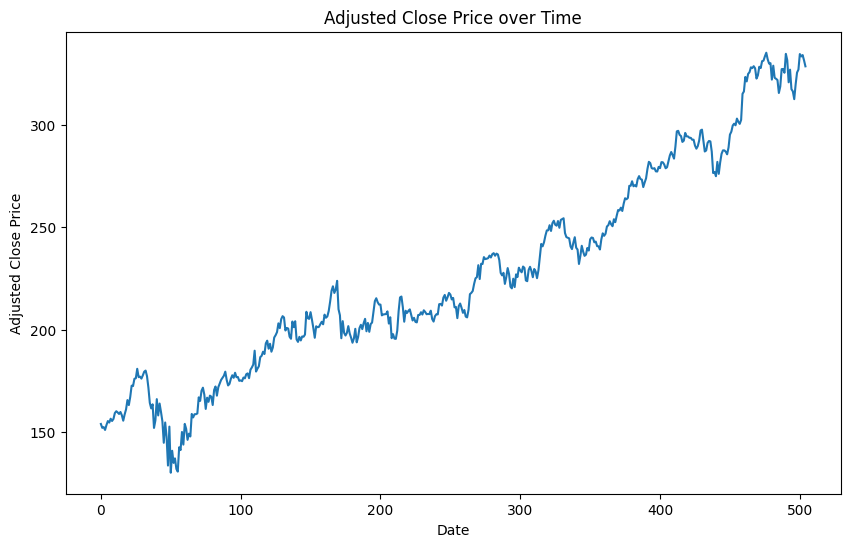
\includegraphics[width=0.6\textwidth]{Week2_adjusted_close_graph.png} % Adjust width as needed
    \caption{Adjusted Closing price vs time}
    \label{fig5}
\end{figure}

\begin{figure}[!h]
    \centering
    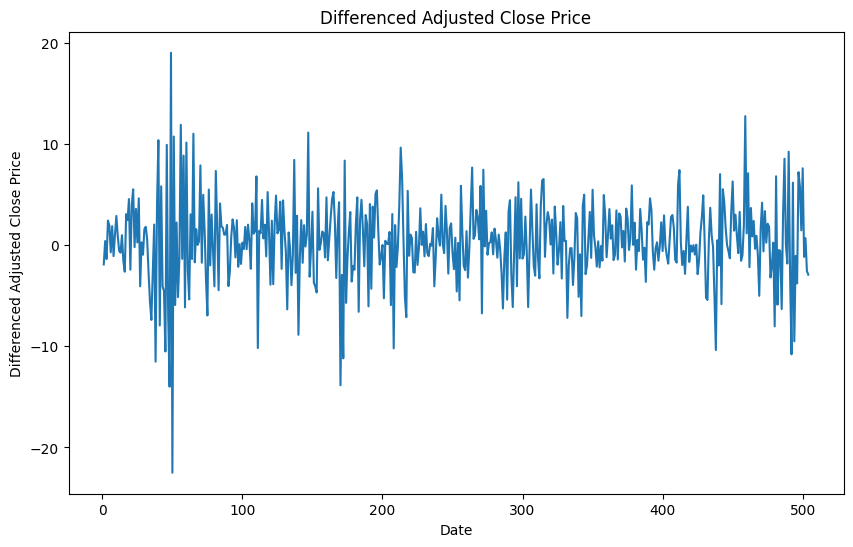
\includegraphics[width=0.6\textwidth]{Week2_differenced_close_graph.png} % Adjust width as needed
    \caption{Differenced closing price vs time for stationality}
    \label{fig6}
\end{figure}

\begin{figure}[!h]
    \centering
    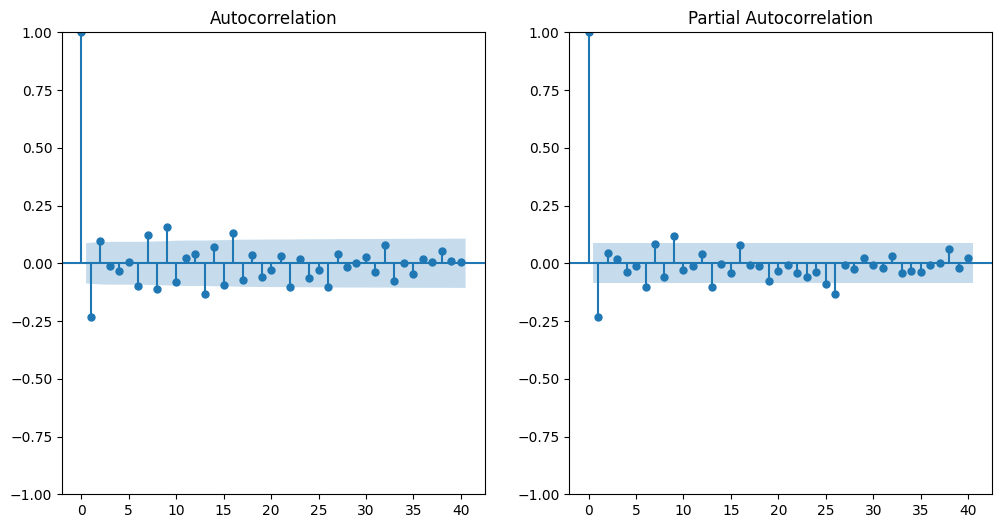
\includegraphics[width=0.6\textwidth]{Week2_correlation_graph.png} % Adjust width as needed
    \caption{Correlation Graph for ARIMA}
    \label{fig7}
\end{figure}

\begin{figure}[!h]
    \centering
    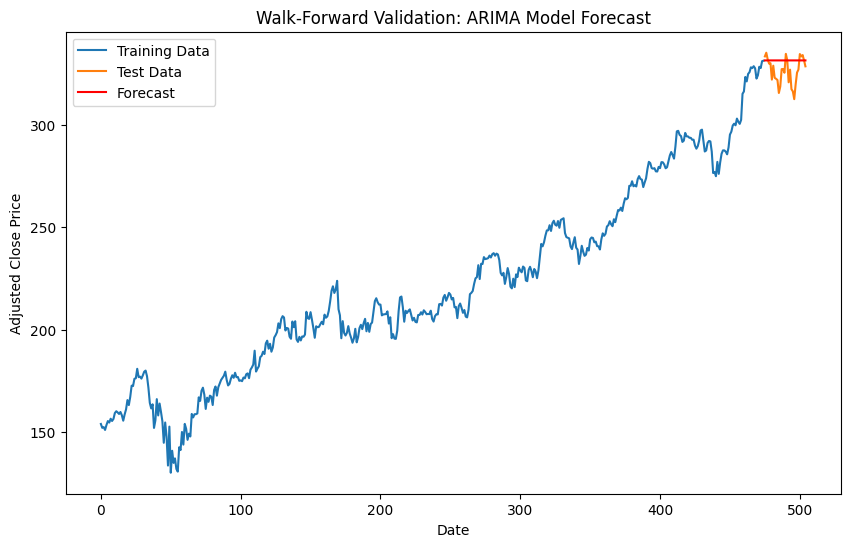
\includegraphics[width=0.6\textwidth]{Week2_final_result.png} % Adjust width as needed
    \caption{Final Results of ARIMA}
    \label{fig8}
\end{figure}

\section{Week 3: Univariate LSTM model and its comparison with ARIMA}
This week focused on exploring LSTM (Long Short-Term Memory) networks and leveraging their power for time series analysis. I began by diving into their architecture, history, and underlying mathematics. After gaining a conceptual understanding, I applied LSTMs to visualize and analyze time series data.

The assignment built upon the previous two weeks by training both an LSTM model and an ARIMA model, comparing their results, and evaluating their strengths and weaknesses. This hands-on approach helped me truly appreciate the capabilities of LSTMs in capturing complex temporal patterns.

While implementing LSTMs using libraries is relatively straightforward, achieving optimal results requires extensive hyperparameter tuning. After fine-tuning, I compared the predictions of ARIMA and LSTM, visualizing the results through various plots. Although the performance wasn’t exceptional, this experiment significantly deepened my understanding and prepared me for the final project.

\begin{figure}[!h]
    \centering
    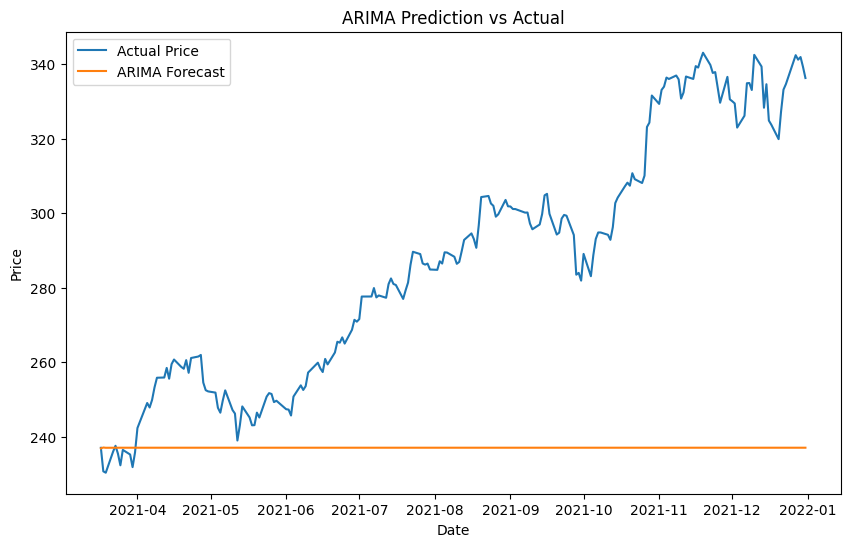
\includegraphics[width=0.5\textwidth]{Week3_ARIMA_prediction.png} % Adjust width as needed
    \caption{ARIMA prediction output}
    \label{fig9}
\end{figure}

\begin{figure}[!h]
    \centering
    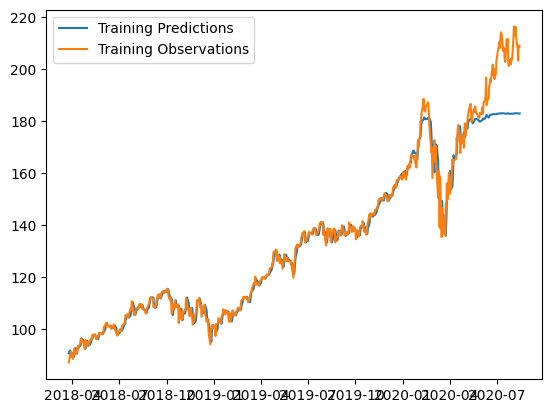
\includegraphics[width=0.5\textwidth]{Week3_LSTM_training.png} % Adjust width as needed
    \caption{LSTM Training output}
    \label{fig10}
\end{figure}

\begin{figure}[!h]
    \centering
    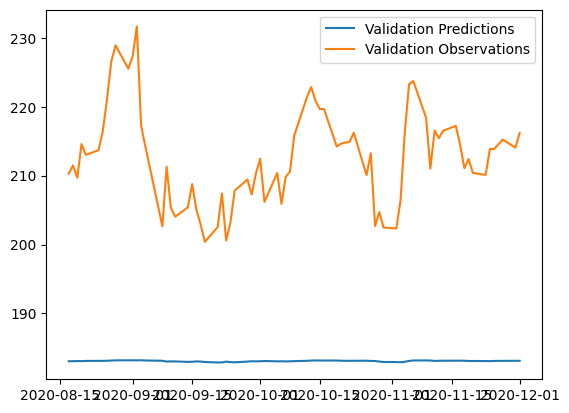
\includegraphics[width=0.5\textwidth]{Week3_LSTM_validation.png} % Adjust width as needed
    \caption{LSTM Validation output}
    \label{fig11}
\end{figure}

\begin{figure}[!h]
    \centering
    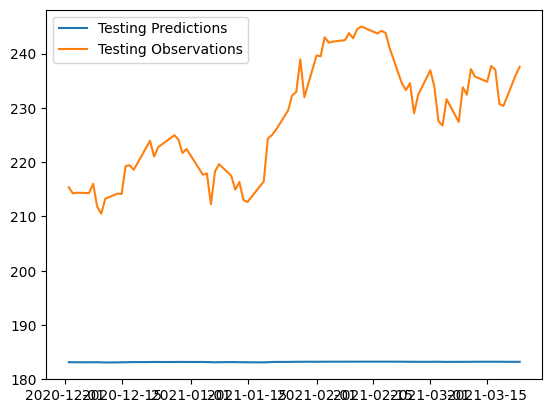
\includegraphics[width=0.5\textwidth]{Week3_LSTM_test.png} % Adjust width as needed
    \caption{LSTM Testing output}
    \label{fig12}
\end{figure}

\begin{figure}[!h]
    \centering
    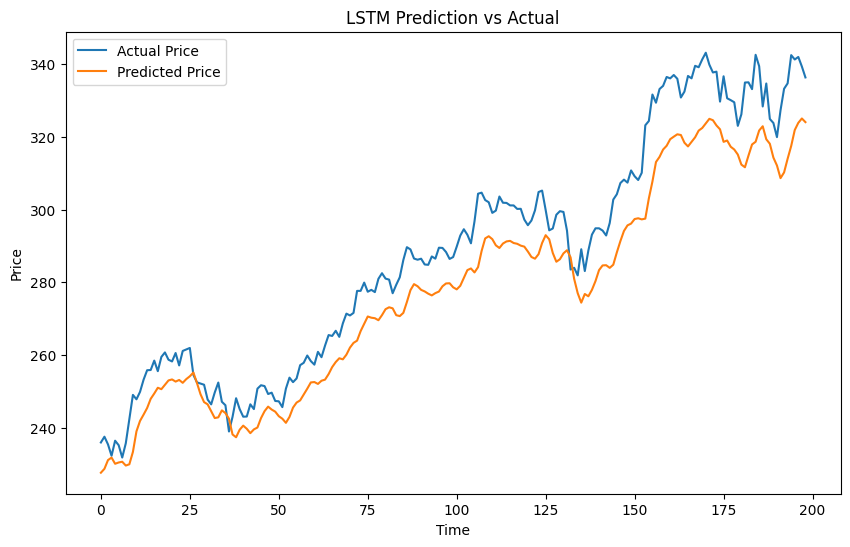
\includegraphics[width=0.5\textwidth]{Week3_LSTM_prediction.png} % Adjust width as needed
    \caption{LSTM Overall Prediction output}
    \label{fig13}
\end{figure}

\newpage

\section{Week 4: Final Project}
The goal of the final project was to integrate market analysis and sentiment analysis to predict stock trends, reinforcing my ability to combine multiple analytical techniques into a unified model. For this, I chose Tesla stock as my target and sourced news data from a Kaggle dataset. After collecting the news, I appended it to the stock price dataset and preprocessed it for sentiment analysis, following the same steps as in Week 2.

For the time series modeling, I used only the polarity score from the sentiment analysis results, excluding subjectivity. The next step was to train an LSTM model using both stock prices and polarity scores as inputs. Given the complexity of the task, training an LSTM wasn’t straightforward, but it provided a more powerful approach than ARIMA, making it the preferred choice for this experiment. Once trained, the model was used to generate predictions based on the provided data.

The final results were not highly accurate, but this project was a valuable learning experience. It gave me deeper insights into the challenges of stock market prediction, sentiment analysis, and LSTM networks. More importantly, it pushed me to code independently, without relying on AI assistance, and made me appreciate the difficulty of forecasting market trends.
\begin{figure}[!h]
    \centering
    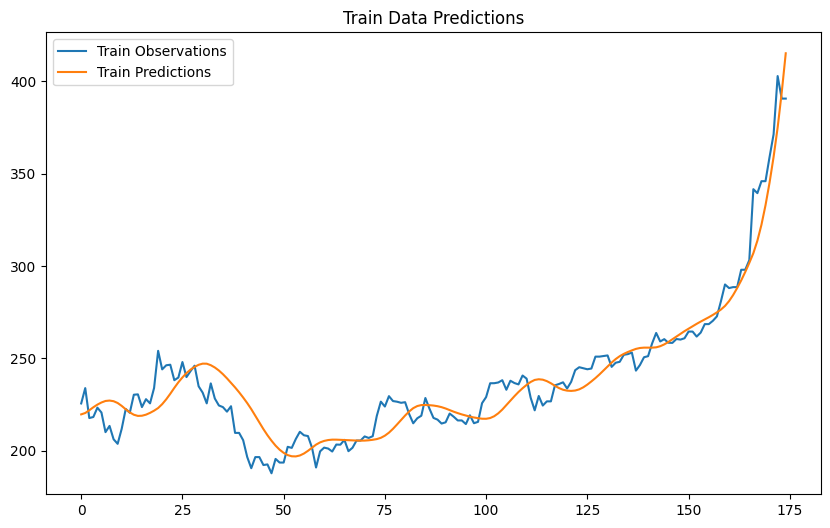
\includegraphics[width=0.5\textwidth]{Week4_train_results.png} % Adjust width as needed
    \caption{Train Result of Final Project}
    \label{fig14}
\end{figure}

\begin{figure}[!h]
    \centering
    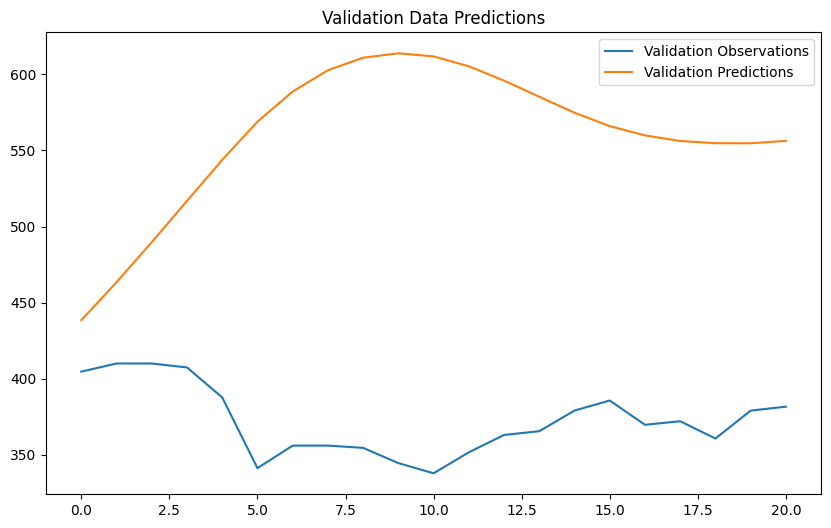
\includegraphics[width=0.5\textwidth]{Week4_validation_results.png} % Adjust width as needed
    \caption{Validation Result of Final Project}
    \label{fig15}
\end{figure}

\begin{figure}[!h]
    \centering
    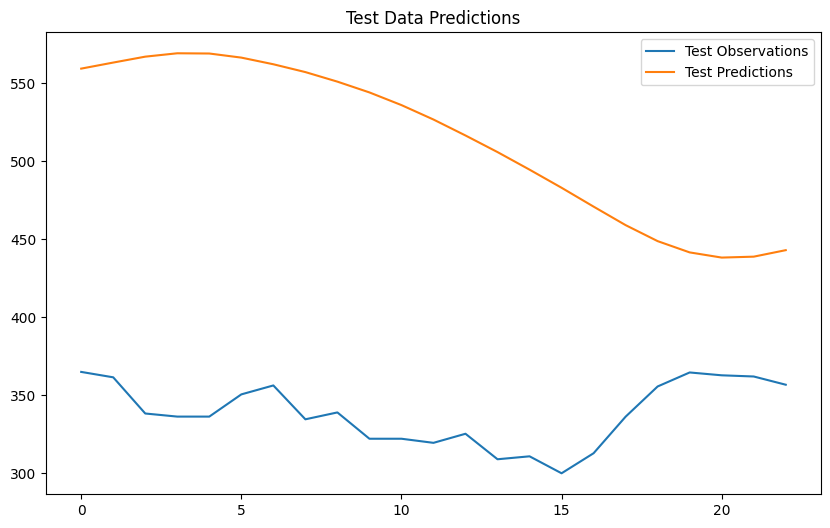
\includegraphics[width=0.5\textwidth]{Week4_test_results.png} % Adjust width as needed
    \caption{Test Result of Final Project}
    \label{fig16}
\end{figure}

\newpage

\section{Conclusions}
In conclusion, combining multivariate LSTMs with sentiment analysis enhances stock trend prediction by capturing both numerical patterns and market sentiment. LSTMs improve forecasting accuracy by handling sequential dependencies, while sentiment analysis extracts insights from news and social media. Despite challenges such as data noise and market volatility, the model demonstrated promising potential.

One key limitation was the infrequency of news updates, which provided only a few instances for the model to learn how sentiment influences stock prices. Additionally, while the LSTM effectively captured trend patterns, its predictions consistently underestimated actual prices by a certain margin, raising questions about whether the model required more training data or better tuning.

Potential improvements include using transformer-based models like BERT for more accurate sentiment analysis, incorporating real-time news feeds and social media trends for richer market signals, optimizing LSTM architectures with attention mechanisms, and experimenting with ensemble models to enhance predictive performance. These advancements could significantly improve the robustness and reliability of stock trend prediction.
\end{document}